% ថ្នាក់ទី ១១ (វិទ្យាសាស្ត្រសង្គម) · ជំពូកទី ៥ · មេរៀនទី ៣ · សៀវភៅ ទំព័រ ១៨៨–២១២
\chapter{អថេរភាពនិងក្រាបនៃអនុគមន៍}

\begin{objBox}[វត្ថុបំណង]
\begin{enumerate}[1]
  \item សិក្សាអថេរភាពនិងសង់ក្រាបនៃអនុគមន៍ពហុធាដឺក្រេទី $3$
  \item សិក្សាអថេរភាពនិងសង់ក្រាបនៃអនុគមន៍ប៊ីការេ
  \item រកអាស៊ីមតូតឈរនិងអាស៊ីមតូតដេកនៃក្រាបតាងអនុគមន៍សនិទាន
  \item សិក្សាអថេរភាពនិងសង់ក្រាបនៃអនុគមន៍សនិទានងាយៗ ។
\end{enumerate}
\end{objBox}

\section{អនុគមន៍ពហុធាដឺក្រេទី 3}
\subsection{អថេរភាពនិងក្រាបនៃអនុគមន៍ពហុធាដឺក្រេទី 3}

\begin{example}[ឧទាហរណ៍ ១]
សិក្សាអថេរភាពនិងសង់ក្រាបនៃ $f(x) = -x^3 - 3x^2 + 4$ ។
\end{example}
\begin{itemize}
  \item \textbf{ដែនកំណត់} ៖ អនុគមន៍ $f$ មានន័យចំពោះគ្រប់ $x \in \mathbb{R}$ គឺ $D = \mathbb{R}$ ។
  \item \textbf{ទិសដៅអថេរភាព} ៖ ដេរីវេ $y' = f'(x) = -3x^2 - 6x = 3x(-x - 2)$ ។ $f'(x) = 0$ សមមូល $3x(-x - 2) = 0$ នាំឱ្យ $x = 0$ ឬ $x = -2$ ។
  \begin{center}
  \begin{tikzpicture}
    \tkzTabInit[lgt=1.6,espcl=2]{$x$ /0.8, $f'(x)$ /0.8}{$-\infty$, $-2$, $0$, $+\infty$}
    \tkzTabLine{, -, z, +, z, -, }
  \end{tikzpicture}
  \end{center}
  \item \textbf{តម្លៃបរមាធៀប} ៖ $f$ មានអប្បបរមាធៀបត្រង់ $x = -2$ ហើយតម្លៃអប្បបរមាធៀបគឺ $y = f(-2) = 0$ ។ $f$ មានអតិបរមាធៀបត្រង់ $x = 0$ ហើយតម្លៃអតិបរមាធៀបគឺ $y = f(0) = 4$ ។
  \item \textbf{លីមីត} ៖ $\displaystyle\lim_{x \to -\infty} f(x) = \lim_{x \to -\infty}\left[x^3\left(-1 - \frac{3}{x} + \frac{4}{x^3}\right)\right] = +\infty$ និង $\displaystyle\lim_{x \to +\infty} f(x) = \lim_{x \to +\infty}\left[x^3\left(-1 - \frac{3}{x} + \frac{4}{x^3}\right)\right] = -\infty$ ។
  \item \textbf{តារាងអថេរភាព}
  \begin{center}
  \begin{tikzpicture}
    \tkzTabInit[lgt=1.6,espcl=2]{$x$ /0.8, $f'(x)$ /0.8, $f(x)$ /1.6}{$-\infty$, $-2$, $0$, $+\infty$}
    \tkzTabLine{, -, z, +, z, -, }
    \tkzTabVar{+/$+\infty$, -/$0$, +/$4$, -/$-\infty$}
  \end{tikzpicture}
  \end{center}
  \item \textbf{ភាពប៉ោង ផត និងចំណុចរបត់} ៖ $f''(x) = -6x - 6$ ។ $f''(x) = 0$ សមមូល $x = -1$ ហើយ $y = f(-1) = 2$ ។ ក្រាបផតលើ $(-\infty, -1)$ ព្រោះ $f'' > 0$ និងប៉ោងលើ $(-1, +\infty)$ ព្រោះ $f'' < 0$ ។ ចំណុច $I(-1, 2)$ ជាចំណុចរបត់ ។
  \item \textbf{ក្រាប} ៖ ចំណុចប្រសព្វរវាងក្រាបនិងអ័ក្ស ។ ក្រាបប្រសព្វអ័ក្ស $(y'oy)$ នោះ $x = 0$ គេបាន $y = 4$ ។ ក្រាបប្រសព្វអ័ក្ស $(x'ox)$ នោះ $y = 0$ គេបាន
  \[ \begin{aligned} -x^3 - 3x^2 + 4 = 0 &\Leftrightarrow -x^3 + x^2 - 4x^2 + 4 = 0\\ &\Leftrightarrow -x^2(x - 1) - 4(x^2 - 1) = 0\\ &\Leftrightarrow -(x - 1)(x + 2)^2 = 0 \end{aligned} \]
  នាំឱ្យ $x = 1$ ឬ $x = -2$ ។
  \item បន្ទាត់ប៉ះត្រង់ចំណុចរបត់ $I(-1, 2)$ មានមេគុណប្រាប់ទិស $f'(-1) = 3$ ។ សមីការបន្ទាត់ប៉ះត្រង់ $I(-1, 2)$ គឺ $y = f'(x_0)(x - x_0) + f(x_0) = 3(x + 1) + 2 = 3x + 5$ ។
  \item \textbf{ផ្ចិតឆ្លុះ} ៖ តាមការបំប្លែងកិលនៃ $\overrightarrow{OI}$ គេបានរូបមន្តប្ដូរតម្រុយ $\begin{cases} x = X + x_0\\ y = Y + y_0 \end{cases} \Rightarrow \begin{cases} x = X - 1\\ y = Y + 2 \end{cases}$ ។ រកសមីការបង្រួម ៖ $Y + 2 = -(X - 1)^3 - 3(X - 1)^2 + 4$ នាំឱ្យសមីការបង្រួម $Y = -X^3 + 3X$ ។ គេបាន $F(-X) = -(-X)^3 + 3(-X) = X^3 - 3X = -(-X^3 + 3X) = -F(X)$ $\Rightarrow Y = F(X) = -X^3 + 3X$ ជាអនុគមន៍សេស ។ ដូច្នេះ ចំណុច $I(-1, 2)$ ជាផ្ចិតឆ្លុះនៃក្រាបតាង $f$ ។
\end{itemize}

\begin{center}
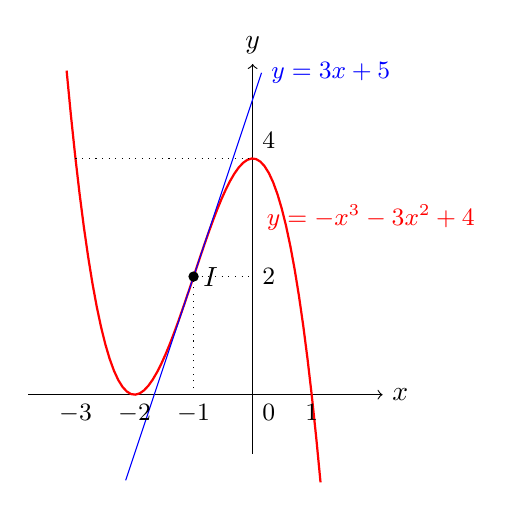
\begin{tikzpicture}[scale=0.75]
  \draw[->] (-3.8,0) -- (2.2,0) node[right] {$x$};
  \draw[->] (0,-1) -- (0,5.6) node[above] {$y$};
  \draw[thick,red,domain=-3.15:1.15,samples=60] plot (\x,{-(\x)^3-3*(\x)^2+4});
  \draw[blue] (-2.15,-1.45) -- (0.15,5.45) node[right] {\small $y = 3x + 5$};
  \fill (-1,2) circle (2.5pt) node[right] {$I$};
  \draw[dotted] (-1,0) -- (-1,2) -- (0,2) node[right] {\small $2$};
  \draw[dotted] (-3,4) -- (0,4);
  \foreach \x in {-3,-2,-1,1} \node[below] at (\x,0) {\small $\x$};
  \node[above right] at (0,4) {\small $4$}; \node[below right] at (0,0) {\small $0$};
  \node[red] at (2,3) {\small $y = -x^3 - 3x^2 + 4$};
\end{tikzpicture}
\end{center}

\begin{example}[ឧទាហរណ៍ ២]
សិក្សាអថេរភាពនិងសង់ក្រាបនៃ $y = x^3 - 3x^2 + 4x - 2$ ។
\end{example}
\begin{itemize}
  \item \textbf{ដែនកំណត់} $D = \mathbb{R}$ ។
  \item \textbf{ទិសដៅអថេរភាព} ៖ ដេរីវេ $y' = 3x^2 - 6x + 4$ ។ បើ $y' = 0$, $3x^2 - 6x + 4 = 0$ មាន $\Delta = -12 < 0$ នាំឱ្យ $\forall x \in \mathbb{R}$, $y' > 0$ ។ ដូច្នេះអនុគមន៍ $y$ កើនជានិច្ចលើ $\mathbb{R}$ ។
  \item \textbf{លីមីត} ៖ $\displaystyle\lim_{x \to -\infty}(x^3 - 3x^2 + 4x - 2) = -\infty$ និង $\displaystyle\lim_{x \to +\infty}(x^3 - 3x^2 + 4x - 2) = +\infty$ ។
  \item \textbf{តារាងអថេរភាព}
  \begin{center}
  \begin{tikzpicture}
    \tkzTabInit[lgt=1.6,espcl=4]{$x$ /0.8, $y'$ /0.8, $y$ /1.6}{$-\infty$, $+\infty$}
    \tkzTabLine{, +, }
    \tkzTabVar{-/$-\infty$, +/$+\infty$}
  \end{tikzpicture}
  \end{center}
  \item \textbf{ភាពប៉ោង ផត និងចំណុចរបត់} ៖ $y'' = 6x - 6$ ។ ក្រាបប៉ោងលើ $(-\infty, 1)$ និងផតលើ $(1, +\infty)$ ហើយមានចំណុចរបត់ $(1, 0)$ ។
  \item \textbf{ក្រាប} ៖ បើ $x = 0$ គេបាន $y = -2$ ។ បើ $y = 0$ គេបាន $x^3 - 3x^2 + 4x - 2 = 0$ ។ ចំពោះ $x = 1$ គេបាន $1^3 - 3\times 1^2 + 4\times 1 - 2 = 0$ ។ គេអាចសរសេរ
  \[
\begin{aligned}
(x^3 - 1^3) - 3(x^2 - 1^2) + 4(x - 1) &= 0\\
&\Leftrightarrow (x - 1)(x^2 - 2x + 2) = 0
\end{aligned}
\]
  នាំឱ្យ $x - 1 = 0$ ឬ $x^2 - 2x + 2 = 0$ ។ ព្រោះ $x^2 - 2x + 2 = 0$ គ្មានឫសជាចំនួនពិត $(\Delta < 0)$ នោះ $x = 1$ ។
  \item បន្ទាត់ប៉ះនឹងក្រាបត្រង់ចំណុចរបត់ $I(1, 0)$ មានមេគុណប្រាប់ទិស $y'(1) = 1$ ។ សមីការបន្ទាត់ប៉ះ $y = 1(x - 1) + 0 = x - 1$ ។
  \item \textbf{ផ្ចិតឆ្លុះ} ៖ តាមការបំប្លែងកិលនៃ $\overrightarrow{OI}$ គេបាន $\begin{cases} x = X + 1\\ y = Y \end{cases}$ ។ សមីការបង្រួម $Y = (X + 1)^3 - 3(X + 1)^2 + 4(X + 1) - 2 = X^3 + X$ ។ $F(-X) = (-X)^3 + (-X) = -(X^3 + X) = -F(X)$ នោះ $F(X)$ ជាអនុគមន៍សេស ។ ដូច្នេះ ចំណុច $I(1, 0)$ ជាផ្ចិតឆ្លុះនៃក្រាប ។
\end{itemize}

\begin{center}
\begin{tikzpicture}[scale=0.8]
  \draw[->] (-1.5,0) -- (3.2,0) node[right] {$x$};
  \draw[->] (0,-2.8) -- (0,2.8) node[above] {$y$};
  \draw[thick,red,domain=-0.05:2.05,samples=60] plot (\x,{(\x)^3-3*(\x)^2+4*\x-2});
  \draw[blue] (-0.8,-1.8) -- (2.8,1.8) node[right] {\small $y = x - 1$};
  \fill (1,0) circle (2.5pt) node[below right] {$I$};
  \draw[dotted] (2,0) -- (2,2) -- (0,2) node[left] {\small $2$};
  \node[left] at (0,-2) {\small $-2$};
  \node[below] at (2,0) {\small $2$};
\end{tikzpicture}
\end{center}

\subsection{អថេរភាពនិងក្រាបនៃអនុគមន៍ \texorpdfstring{$y = ax^3 + bx^2 + cx + d$}{y = ax3 + bx2 + cx + d}}

\begin{itemize}
  \item ដែនកំណត់ $D = \mathbb{R}$ ។
  \item ទិសដៅអថេរភាព ៖ $y' = 3ax^2 + 2bx + c$ ។ បើ $y' = 0$ មានឫសពីរផ្សេងគ្នាជាចំនួនពិត នោះអនុគមន៍មានអតិបរមាធៀបមួយនិងអប្បបរមាធៀបមួយ ។ បើ $y' = 0$ មានឫសឌុបឬគ្មានឫសជាចំនួនពិត នោះអនុគមន៍គ្មានបរមាធៀបទេ ។
  \item លីមីត ៖ $\displaystyle\lim_{x \to -\infty}(ax^3 + bx^2 + cx + d) = \begin{cases} -\infty & \text{បើ } a > 0\\ +\infty & \text{បើ } a < 0 \end{cases}$ និង $\displaystyle\lim_{x \to +\infty}(ax^3 + bx^2 + cx + d) = \begin{cases} +\infty & \text{បើ } a > 0\\ -\infty & \text{បើ } a < 0 \end{cases}$ ។
  \item តារាងអថេរភាព (ករណី $y' = 0$ មានឫសពីរផ្សេងគ្នា $x_1 < x_2$) ៖
  \begin{center}
  \begin{tikzpicture}
    \tkzTabInit[lgt=1.4,espcl=1.6]{$x$ /0.7, $y'$ /0.7, $y$ /1.4}{$-\infty$, $x_1$, $x_2$, $+\infty$}
    \tkzTabLine{, +, z, -, z, +, }
    \tkzTabVar{-/$-\infty$, +/$y_1$, -/$y_2$, +/$+\infty$}
  \end{tikzpicture}
  \quad
  \begin{tikzpicture}
    \tkzTabInit[lgt=1.4,espcl=1.6]{$x$ /0.7, $y'$ /0.7, $y$ /1.4}{$-\infty$, $x_1$, $x_2$, $+\infty$}
    \tkzTabLine{, -, z, +, z, -, }
    \tkzTabVar{+/$+\infty$, -/$y_1$, +/$y_2$, -/$-\infty$}
  \end{tikzpicture}

  \small (ឆ្វេង ៖ $a > 0$ \qquad ស្ដាំ ៖ $a < 0$)
  \end{center}
  បើ $y' = 0$ មានឫសឌុប ឬគ្មានឫស នោះ $y$ កើនជានិច្ច (បើ $a > 0$) ឬចុះជានិច្ច (បើ $a < 0$) ។
  \item ចំណុចរបត់ ៖ $y'' = 6ax + 2b$ ។ ក្រាបតាងអនុគមន៍មានចំណុចរបត់ $I\left(-\dfrac{b}{3a}, y\left(-\dfrac{b}{3a}\right)\right)$ ហើយដែលជាផ្ចិតឆ្លុះនៃក្រាប ។
\end{itemize}

\begin{center}
\begin{tikzpicture}[scale=0.55]
  \foreach \i/\f/\lab in {0/{0.3*\x*\x*\x-1.2*\x}/{$a > 0$, $y'$ មានឫសពីរ},1/{-0.3*\x*\x*\x+1.2*\x}/{$a < 0$, $y'$ មានឫសពីរ},2/{0.25*\x*\x*\x+0.4*\x}/{$a > 0$, $y'$ គ្មានឫស},3/{-0.25*\x*\x*\x-0.4*\x}/{$a < 0$, $y'$ គ្មានឫស}} {
    \begin{scope}[xshift=\i*6.5cm]
      \draw[->] (-2.6,0) -- (2.6,0) node[right] {\small $x$};
      \draw[->] (0,-2.6) -- (0,2.6) node[above] {\small $y$};
      \draw[thick,green!50!black,domain=-2.4:2.4,samples=50] plot (\x,{\f});
      \node at (0,-3.3) {\small \lab};
    \end{scope}
  }
\end{tikzpicture}
\end{center}

\begin{pro}
សិក្សាអថេរភាពនិងសង់ក្រាបតាងអនុគមន៍ខាងក្រោម ៖ \quad ក. $y = -x^3 + x^2 - x - 1$ \quad ខ. $y = 2x^3 - 3x^2 + 1$ ។
\ans
ក. $y' = -3x^2 + 2x - 1 < 0$ ជានិច្ច ($\Delta' = -2 < 0$) ៖ អនុគមន៍ចុះជានិច្ចលើ $\mathbb{R}$ ។ ចំណុចរបត់ $\left(\dfrac{1}{3}, -\dfrac{34}{27}\right)$ ។

ខ. $y' = 6x(x - 1)$ ៖ អតិបរមាធៀប $y(0) = 1$, អប្បបរមាធៀប $y(1) = 0$ ។ ចំណុចរបត់ $\left(\dfrac{1}{2}, \dfrac{1}{2}\right)$ ។
\end{pro}

\section{អនុគមន៍ប៊ីការេ}
\subsection{អថេរភាពនិងក្រាបនៃអនុគមន៍ប៊ីការេ}

\begin{example}[ឧទាហរណ៍]
សិក្សាអថេរភាពនិងសង់ក្រាបនៃ $y = -x^4 + 2x^2 - 2$ ។
\end{example}
\begin{itemize}
  \item \textbf{ដែនកំណត់} $D = \mathbb{R}$ ។
  \item \textbf{ទិសដៅអថេរភាព} ៖ ដេរីវេ $y' = -4x^3 + 4x = -4x(x^2 - 1)$ ។ បើ $y' = 0$ ៖ $-4x(x^2 - 1) = 0 \Rightarrow x = 0$ ឬ $x = \pm 1$ ។
  \begin{center}
  \begin{tikzpicture}
    \tkzTabInit[lgt=1.6,espcl=1.8]{$x$ /0.8, $-4x$ /0.8, $x^2 - 1$ /0.8, $y'$ /0.8}{$-\infty$, $-1$, $0$, $1$, $+\infty$}
    \tkzTabLine{, +, t, +, z, -, t, -, }
    \tkzTabLine{, +, z, -, t, -, z, +, }
    \tkzTabLine{, +, z, -, z, +, z, -, }
  \end{tikzpicture}
  \end{center}
  \item \textbf{តម្លៃបរមាធៀប} ៖ អនុគមន៍មានអតិបរមាធៀបពីរត្រង់ $x = -1$ និង $x = 1$ ហើយតម្លៃអតិបរមាធៀប $y(-1) = y(1) = -1$ ។ អប្បបរមាធៀបមួយត្រង់ $x = 0$ ហើយតម្លៃអប្បបរមាធៀប $y(0) = -2$ ។
  \item \textbf{លីមីត} ៖ $\displaystyle\lim_{x \to \pm\infty} y = \lim_{x \to \pm\infty} x^4\left(-1 + \frac{2}{x^2} - \frac{2}{x^4}\right) = -\infty$ ។
  \item \textbf{តារាងអថេរភាព}
  \begin{center}
  \begin{tikzpicture}
    \tkzTabInit[lgt=1.6,espcl=1.8]{$x$ /0.8, $y'$ /0.8, $y$ /1.6}{$-\infty$, $-1$, $0$, $1$, $+\infty$}
    \tkzTabLine{, +, z, -, z, +, z, -, }
    \tkzTabVar{-/$-\infty$, +/$-1$, -/$-2$, +/$-1$, -/$-\infty$}
  \end{tikzpicture}
  \end{center}
  \item \textbf{ភាពប៉ោង ផត និងចំណុចរបត់} ៖ $y'' = -12x^2 + 4$ ។ បើ $y'' = 0$, $x = \pm\dfrac{\sqrt{3}}{3}$ ហើយ $y\left(\pm\dfrac{\sqrt{3}}{3}\right) = -\dfrac{13}{9}$ ។ ក្រាបប៉ោងលើ $\left(-\infty, -\dfrac{\sqrt{3}}{3}\right)$ និង $\left(\dfrac{\sqrt{3}}{3}, +\infty\right)$, ផតលើ $\left(-\dfrac{\sqrt{3}}{3}, \dfrac{\sqrt{3}}{3}\right)$ ។ ចំណុចរបត់ $\left(-\dfrac{\sqrt{3}}{3}, -\dfrac{13}{9}\right)$ និង $\left(\dfrac{\sqrt{3}}{3}, -\dfrac{13}{9}\right)$ ។
  \item \textbf{ក្រាប} ៖ ក្រាបប្រសព្វអ័ក្សអរដោនេនោះ $x = 0$ គេបាន $y = -2$ ។ ក្រាបប្រសព្វអ័ក្សអាប់ស៊ីសនោះ $y = 0$ គេបាន $-x^4 + 2x^2 - 2 = 0$ ។ តាង $t = x^2$ $(t \ge 0)$ គេបាន $-t^2 + 2t - 2 = 0$, $\Delta' = -1 < 0$ សមីការគ្មានឫសជាចំនួនពិត ហើយក្រាបមិនជួបអ័ក្ស $x'ox$ ទេ ។
  \item \textbf{អ័ក្សឆ្លុះ} ៖ គេបាន $y(-x) = -(-x)^4 + 2(-x)^2 - 2 = -x^4 + 2x^2 - 2 = y(x)$ $\Rightarrow y$ ជាអនុគមន៍គូ នោះអ័ក្សអរដោនេ $(y'oy)$ ជាអ័ក្សឆ្លុះនៃក្រាប ។
  \item តារាងតម្លៃលេខ ៖ $y\left(\pm\dfrac{3}{2}\right) = -\dfrac{41}{16} \approx -2.5$ ។
\end{itemize}

\begin{center}
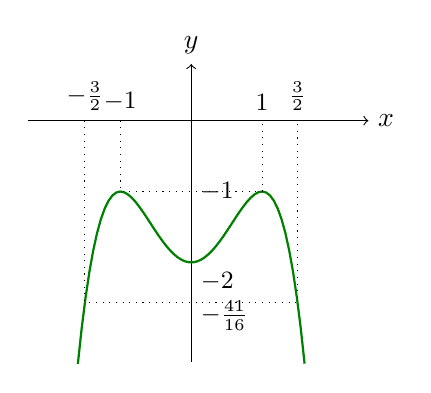
\begin{tikzpicture}[scale=0.9]
  \draw[->] (-2.3,0) -- (2.5,0) node[right] {$x$};
  \draw[->] (0,-3.4) -- (0,0.8) node[above] {$y$};
  \draw[thick,green!50!black,domain=-1.6:1.6,samples=60] plot (\x,{-(\x)^4+2*(\x)^2-2});
  \draw[dotted] (-1,0) -- (-1,-1) -- (1,-1) -- (1,0);
  \draw[dotted] (-1.5,0) -- (-1.5,-2.5625) -- (1.5,-2.5625) -- (1.5,0);
  \foreach \x in {-1,1} \node[above] at (\x,0) {\small $\x$};
  \node[above] at (-1.5,0) {\small $-\frac{3}{2}$}; \node[above] at (1.5,0) {\small $\frac{3}{2}$};
  \node[right] at (0,-1) {\small $-1$}; \node[below right] at (0,-2) {\small $-2$};
  \node[right] at (0,-2.75) {\small $-\frac{41}{16}$};
\end{tikzpicture}
\end{center}

\subsection{អថេរភាពនិងក្រាបនៃ \texorpdfstring{$y = ax^4 + bx^2 + c$}{y = ax4 + bx2 + c}}

\begin{itemize}
  \item ដែនកំណត់ $D = \mathbb{R}$ ។
  \item ទិសដៅអថេរភាព ៖ $y' = 4ax^3 + 2bx = 2x(2ax^2 + b)$ ។ $y' = 0$ មានឫសតែមួយគត់ជាចំនួនពិត ($x = 0$) បើ $\dfrac{b}{a} \ge 0$ ។ $y' = 0$ មានឫសបីផ្សេងគ្នាជាចំនួនពិត បើ $\dfrac{b}{a} < 0$ ។
  \item លីមីត ៖ $\displaystyle\lim_{x \to \pm\infty} y = \lim_{x \to \pm\infty} ax^4\left(1 + \frac{b}{ax^2} + \frac{c}{ax^4}\right) = \begin{cases} +\infty & \text{បើ } a > 0\\ -\infty & \text{បើ } a < 0 \end{cases}$ ។
  \item ចំណុចរបត់ ៖ $y'' = 12ax^2 + 2b$ ។ $y'' = 0$ គ្មានឫស ឬមានឫសឌុបជាចំនួនពិត បើ $\dfrac{b}{a} \ge 0$ ហើយក្រាបគ្មានចំណុចរបត់ ។ $y'' = 0$ មានឫសពីរផ្សេងគ្នាជាចំនួនពិត បើ $\dfrac{b}{a} < 0$ ហើយក្រាបមានចំណុចរបត់ពីរ ។
  \item ក្រាប ៖ អ័ក្សអរដោនេ ជាអ័ក្សឆ្លុះនៃក្រាប ។
\end{itemize}

\begin{center}
\begin{tikzpicture}[scale=0.55]
  \foreach \i/\f/\lab in {0/{0.25*(\x)^4+0.5*(\x)^2-1.5}/{$a > 0$, $\frac{b}{a} \ge 0$},1/{-0.25*(\x)^4-0.5*(\x)^2+1.5}/{$a < 0$, $\frac{b}{a} \ge 0$},2/{0.3*(\x)^4-1.4*(\x)^2+0.5}/{$a > 0$, $\frac{b}{a} < 0$},3/{-0.3*(\x)^4+1.4*(\x)^2-0.5}/{$a < 0$, $\frac{b}{a} < 0$}} {
    \begin{scope}[xshift=\i*6.5cm]
      \draw[->] (-2.6,0) -- (2.6,0) node[right] {\small $x$};
      \draw[->] (0,-2.6) -- (0,2.6) node[above] {\small $y$};
      \draw[thick,red,domain=-2.35:2.35,samples=50] plot (\x,{\f});
      \node at (0,-3.3) {\small \lab};
    \end{scope}
  }
\end{tikzpicture}
\end{center}

\begin{pro}
សិក្សាអថេរភាពនិងសង់ក្រាបនៃអនុគមន៍ខាងក្រោម ៖ \quad ក. $y = -x^4 - x^2 + 2$ \quad ខ. $y = x^4 - 2x^2 + 1$ ។
\ans
ក. $y' = -2x(2x^2 + 1)$ ៖ កើនលើ $(-\infty, 0)$ ចុះលើ $(0, +\infty)$ ៖ អតិបរមា $y(0) = 2$ ។ គ្មានចំណុចរបត់ ។ ក្រាបកាត់អ័ក្ស $x'ox$ ត្រង់ $x = \pm 1$ ។

ខ. $y' = 4x(x^2 - 1)$ ៖ អប្បបរមាធៀប $y(\pm 1) = 0$, អតិបរមាធៀប $y(0) = 1$ ។ ចំណុចរបត់ $\left(\pm\dfrac{\sqrt{3}}{3}, \dfrac{4}{9}\right)$ ។
\end{pro}

\section{អនុគមន៍សនិទាន}

ក្នុងផ្នែកនេះ យើងសិក្សាអនុគមន៍សនិទាន $y = \dfrac{ax + b}{cx + d}$ ដែល $c \ne 0$ និង $ad - bc \ne 0$ ។
\subsection{អាស៊ីមតូតនៃក្រាប}

\begin{definition}[និយមន័យ]
បន្ទាត់ $L$ ជាអាស៊ីមតូតនៃក្រាប $C$ តាងអនុគមន៍ $y = f(x)$ កាលណាចម្ងាយ $MH$ ពីចំណុច $M$ នៃ $C$ ទៅបន្ទាត់ $L$ ខិតជិតសូន្យ នៅពេលចំណុច $M$ រត់លើក្រាប $C$ ខិតទៅជិតអនន្ត ។
\end{definition}

\subsubsection{អាស៊ីមតូតឈរ}

\begin{example}[ឧទាហរណ៍]
គេឱ្យអនុគមន៍ $y = \dfrac{1}{x - 2}$ និងតារាងតម្លៃលេខ
\[
\begin{array}{c|ccc|c|ccc}
x & 1.99 & 1.999 & 1.9999 & 2 & 2.0001 & 2.001 & 2.01\\ \hline
y = \frac{1}{x - 2} & -10^2 & -10^3 & -10^4 & \| & 10^4 & 10^3 & 10^2
\end{array}
\]
\end{example}
តាមតារាងតម្លៃលេខខាងលើ បើ $x$ យកតម្លៃកាន់តែជិត $2$ ពីខាងឆ្វេង នោះអនុគមន៍មានតម្លៃអវិជ្ជមាន ហើយកាន់តែតូចទៅៗគ្មានទីបញ្ចប់ ។ គេបាន $\displaystyle\lim_{x \to 2^-} y = -\infty$ ។ ម្យ៉ាងទៀតបើ $x$ យកតម្លៃកាន់តែជិត $2$ ពីខាងស្ដាំនោះ អនុគមន៍មានតម្លៃវិជ្ជមានកាន់តែធំទៅៗគ្មានទីបញ្ចប់ ។ គេបាន $\displaystyle\lim_{x \to 2^+} y = +\infty$ ។

ក្នុងករណីទាំងពីរនេះ ចម្ងាយ $MH$ ពីចំណុច $M$ ទៅបន្ទាត់មានសមីការ $x = 2$ ខិតជិតសូន្យ កាលណាចំណុច $M$ រត់លើក្រាបខិតទៅជិតអនន្ត ។ គេថាបន្ទាត់មានសមីការ $x = 2$ ជាអាស៊ីមតូតឈរនៃក្រាបតាងអនុគមន៍ ។

\begin{center}
\begin{tikzpicture}[scale=0.7]
  \draw[->] (-1.5,0) -- (5.5,0) node[right] {$x$};
  \draw[->] (0,-3.5) -- (0,3.5) node[above] {$y$};
  \draw[dashed] (2,-3.5) -- (2,3.5) node[above] {\small $x = 2$};
  \draw[thick,green!50!black,domain=-1.4:1.7,samples=50] plot (\x,{1/(\x-2)});
  \draw[thick,green!50!black,domain=2.3:5.3,samples=50] plot (\x,{1/(\x-2)});
\end{tikzpicture}
\end{center}

\begin{formulaBox}[ជាទូទៅ]
បន្ទាត់ $L$ មានសមីការ $x = x_0$ ជាអាស៊ីមតូតឈរនៃក្រាបតាងអនុគមន៍ $y = f(x)$ កាលណា $\displaystyle\lim_{x \to x_0} f(x) = \pm\infty$ (ពីខាងឆ្វេង ឬពីខាងស្ដាំ) ។
\end{formulaBox}

\begin{example}[លំហាត់គំរូ]
រកសមីការអាស៊ីមតូតឈរនៃក្រាបតាង $y = \dfrac{2x - 1}{x + 1}$ ។
\end{example}
\ans
ជំហានទី $1$ ៖ រកតម្លៃឫសនៃភាគបែង ៖ $x + 1 = 0 \Leftrightarrow x = -1$ ។

ជំហានទី $2$ ៖ រកលីមីតខាងស្ដាំនិងខាងឆ្វេងត្រង់ $x = -1$ ។ គេបាន
\[
\begin{aligned}
\lim_{x \to -1^+}\frac{2x - 1}{x + 1} &= -\infty \text{ ព្រោះ } \lim_{x \to -1^+}(2x - 1)\\
&= -3, \ \lim_{x \to -1^+}(x + 1) = 0^+
\end{aligned}
\]
\[
\begin{aligned}
\lim_{x \to -1^-}\frac{2x - 1}{x + 1} &= +\infty \text{ ព្រោះ } \lim_{x \to -1^-}(2x - 1)\\
&= -3, \ \lim_{x \to -1^-}(x + 1) = 0^-
\end{aligned}
\]
ដូច្នេះ បន្ទាត់ $L : x = -1$ ជាអាស៊ីមតូតឈរនៃក្រាប ។

\begin{note}[សម្គាល់]
បើភាគបែងនៃអនុគមន៍ប្រភាគសនិទានមានឫស $x_0$ (ហើយភាគយកមិនសូន្យត្រង់ $x_0$) នោះបន្ទាត់មានសមីការ $x = x_0$ ជាអាស៊ីមតូតឈរនៃក្រាប ។
\end{note}

\begin{pro}
រកអាស៊ីមតូតឈរនៃក្រាបតាងអនុគមន៍ខាងក្រោមនេះ ៖ \quad ក. $y = \dfrac{2(x + 1)}{x - 1}$ \quad ខ. $y = \dfrac{x^2}{x + 2}$ ។
\ans
ក. $x = 1$ \quad ខ. $x = -2$ ។
\end{pro}

\subsubsection{អាស៊ីមតូតដេក}

\begin{example}[ឧទាហរណ៍]
គេឱ្យអនុគមន៍ $y = f(x) = \dfrac{-2x}{x - 1}$ ។ គេអាចសរសេរ $f(x) = \dfrac{-2x}{x\left(1 - \frac{1}{x}\right)} = \dfrac{-2}{1 - \frac{1}{x}}$, $x \ne 0$ ។
\[
\begin{gathered}
\lim_{x \to -\infty} f(x) = -2,\\
\lim_{x \to +\infty} f(x) = -2\\
\text{ព្រោះ } \lim_{x \to \pm\infty}\frac{1}{x} = 0
\end{gathered}
\]
\end{example}
ក្នុងករណីនេះ ចម្ងាយ $MH$ ពីចំណុច $M$ ទៅបន្ទាត់ $L : y = -2$ ខិតជិតសូន្យ កាលណាចំណុច $M$ រត់លើក្រាបនៃ $f$ ទៅអនន្ត ។ គេថាបន្ទាត់ $L : y = -2$ ជាអាស៊ីមតូតដេកនៃក្រាបតាង $f$ ។

\begin{center}
\begin{tikzpicture}[scale=0.6]
  \draw[->] (-4,0) -- (5,0) node[right] {$x$};
  \draw[->] (0,-6) -- (0,3) node[above] {$y$};
  \draw[dashed] (1,-6) -- (1,3);
  \draw[dashed] (-4,-2) -- (5,-2) node[right] {\small $L : y = -2$};
  \draw[thick,green!50!black,domain=-3.8:0.75,samples=50] plot (\x,{-2*\x/(\x-1)});
  \draw[thick,green!50!black,domain=1.4:4.8,samples=50] plot (\x,{-2*\x/(\x-1)});
  \node[below right] at (1,0) {\small $1$}; \node[below left] at (0,0) {\small $0$};
\end{tikzpicture}
\end{center}

\begin{formulaBox}[ជាទូទៅ]
បន្ទាត់ $L$ មានសមីការ $y = b$ ជាអាស៊ីមតូតដេកនៃក្រាបតាងអនុគមន៍ $y = f(x)$ កាលណា $\displaystyle\lim_{x \to +\infty} f(x) = b$ ឬ $\displaystyle\lim_{x \to -\infty} f(x) = b$, $b \in \mathbb{R}$ ។
\end{formulaBox}

\begin{example}[លំហាត់គំរូ]
រកអាស៊ីមតូតដេកនៃក្រាបតាង $y = \dfrac{2x + 3}{x - 1}$ ។
\end{example}
\ans
ជំហានទី $1$ ៖ ពិនិត្យដឺក្រេនៃភាគយកនិងភាគបែង ។ ដឺក្រេភាគយក ស្មើដឺក្រេភាគបែង ដូច្នេះក្រាបតាងអនុគមន៍មានអាស៊ីមតូតដេក ។

ជំហានទី $2$ ៖ រកលីមីតនៃអនុគមន៍នៅត្រង់អនន្ត ៖ $\dfrac{2x + 3}{x - 1} = \dfrac{x\left(2 + \frac{3}{x}\right)}{x\left(1 - \frac{1}{x}\right)} = \dfrac{2 + \frac{3}{x}}{1 - \frac{1}{x}}$ $(x \ne 0)$
\[
\begin{gathered}
\lim_{x \to \pm\infty} y = \lim_{x \to \pm\infty}\frac{2 + \frac{3}{x}}{1 - \frac{1}{x}} = 2\\
\text{ព្រោះ} \quad \lim_{x \to \pm\infty}\frac{1}{x} = 0
\end{gathered}
\]
ដូច្នេះ បន្ទាត់មានសមីការ $y = 2$ ជាអាស៊ីមតូតដេកនៃក្រាប ។

\begin{note}[សម្គាល់]
បើដឺក្រេភាគយកតូចជាងឬស្មើដឺក្រេភាគបែង នោះក្រាបនៃអនុគមន៍សនិទានមានអាស៊ីមតូតដេក ហើយក្រៅពីនេះក្រាបគ្មានអាស៊ីមតូតដេកទេ ។
\end{note}

\begin{pro}
រកអាស៊ីមតូតដេកនៃក្រាបតាងអនុគមន៍ខាងក្រោម ៖ \quad ក. $y = \dfrac{x + 2}{1 - 2x}$ \quad ខ. $y = \dfrac{x - 1}{x^2 + 1}$ ។
\ans
ក. $y = -\dfrac{1}{2}$ \quad ខ. $y = 0$ ។
\end{pro}

\subsection{អថេរភាពនិងក្រាបនៃអនុគមន៍ \texorpdfstring{$y = \frac{ax + b}{cx + d}$}{y = (ax+b)/(cx+d)}}

\begin{example}[ឧទាហរណ៍]
សិក្សាអថេរភាពនិងសង់ក្រាបនៃ $f(x) = \dfrac{2x - 1}{x + 1}$ ។
\end{example}
\begin{itemize}
  \item \textbf{ដែនកំណត់} ៖ អនុគមន៍ $f$ មានន័យកាលណា $x \ne -1$ គឺ $D = \mathbb{R} - \{-1\}$ ។
  \item \textbf{ទិសដៅអថេរភាព} ៖ ដេរីវេ $f'(x) = \dfrac{(2x - 1)'(x + 1) - (2x - 1)(x + 1)'}{(x + 1)^2} = \dfrac{3}{(x + 1)^2}$ ។ ដោយ $(x + 1)^2 > 0$ ចំពោះគ្រប់ $x \in D$ នោះ $f'(x) > 0$ ចំពោះគ្រប់ $x \in D$ ។ $f$ ជាអនុគមន៍កើនជានិច្ចលើ $D$ ហើយគ្មានបរមាទេ ។
  \item \textbf{លីមីតនិងអាស៊ីមតូត} ៖ $\displaystyle\lim_{x \to -1^-} f(x) = +\infty$ និង $\displaystyle\lim_{x \to -1^+} f(x) = -\infty$ ។ ដូច្នេះ បន្ទាត់មានសមីការ $x = -1$ ជាអាស៊ីមតូតឈរនៃក្រាប ។
  \[ \lim_{x \to \pm\infty} f(x) = \lim_{x \to \pm\infty}\frac{x\left(2 - \frac{1}{x}\right)}{x\left(1 + \frac{1}{x}\right)} = \lim_{x \to \pm\infty}\frac{2 - \frac{1}{x}}{1 + \frac{1}{x}} = 2 \]
  ដូច្នេះ បន្ទាត់មានសមីការ $y = 2$ ជាអាស៊ីមតូតដេកនៃក្រាប ។
  \item \textbf{តារាងអថេរភាព}
  \begin{center}
  \begin{tikzpicture}
    \tkzTabInit[lgt=1.6,espcl=2.5]{$x$ /0.8, $f'(x)$ /0.8, $f(x)$ /1.6}{$-\infty$, $-1$, $+\infty$}
    \tkzTabLine{, +, d, +, }
    \tkzTabVar{-/$2$, +D-/$+\infty$/$-\infty$, +/$2$}
  \end{tikzpicture}
  \end{center}
  \item \textbf{ក្រាប} ៖ ចំណុចប្រសព្វរវាងក្រាបនិងអ័ក្ស ៖ $x = 0$ គេបាន $y = -1$ និង $y = 0$ គេបាន $2x - 1 = 0 \Leftrightarrow x = \dfrac{1}{2}$ ។
  \item \textbf{ផ្ចិតឆ្លុះនៃក្រាប} ៖ អាស៊ីមតូតទាំងពីរកាត់គ្នាត្រង់ចំណុច $S(-1, 2)$ ។ តាមការបំប្លែងកិលវិចទ័រ $\overrightarrow{OS}$ គេបានរូបមន្តប្ដូរតម្រុយ $\begin{cases} x = X - 1\\ y = Y + 2 \end{cases}$ ។ គេមាន $Y + 2 = \dfrac{2(X - 1) - 1}{X - 1 + 1} = \dfrac{2X - 3}{X} = 2 - \dfrac{3}{X}$ ។ សមីការបង្រួម $Y = -\dfrac{3}{X}$ ជាអនុគមន៍សេស ព្រោះ $F(-X) = \dfrac{3}{X} = -F(X)$ ។ ដូច្នេះ $S(-1, 2)$ ជាផ្ចិតឆ្លុះនៃក្រាបតាងអនុគមន៍ ។
\end{itemize}

\begin{center}
\begin{tikzpicture}[scale=0.55]
  \draw[->] (-6,0) -- (5,0) node[right] {$x$};
  \draw[->] (0,-4) -- (0,7) node[above] {$y$};
  \draw[dashed] (-1,-4) -- (-1,7);
  \draw[dashed] (-6,2) -- (5,2) node[above] {\small $y = 2$};
  \draw[thick,green!50!black,domain=-6:-1.5,samples=50] plot (\x,{(2*\x-1)/(\x+1)});
  \draw[thick,green!50!black,domain=-0.55:5,samples=50] plot (\x,{(2*\x-1)/(\x+1)});
  \fill (-1,2) circle (3pt) node[above left] {$S$};
  \node[below right] at (0.5,0) {\small $\frac{1}{2}$}; \node[right] at (0,-1) {\small $-1$};
\end{tikzpicture}
\end{center}

\begin{formulaBox}[ករណីទូទៅ]
សិក្សាអថេរភាពនិងក្រាបនៃ $y = \dfrac{ax + b}{cx + d}$ ដែល $c \ne 0$ និង $ad - bc \ne 0$ ។
\begin{itemize}
  \item ដែនកំណត់ ៖ $D = \mathbb{R} - \left\{-\dfrac{d}{c}\right\}$ ។
  \item ទិសដៅអថេរភាព ៖ ដេរីវេ $y' = \dfrac{ad - bc}{(cx + d)^2}$ ។ បើ $ad - bc > 0$ នោះ $y' > 0$ ហើយអនុគមន៍កើនលើ $D$ និងគ្មានបរមា ។ បើ $ad - bc < 0$ នោះ $y' < 0$ ហើយអនុគមន៍ចុះលើ $D$ និងគ្មានបរមា ។
  \item លីមីតនិងអាស៊ីមតូត ៖ ដោយ $\displaystyle\lim_{x \to (-\frac{d}{c})^{\pm}} f(x) = \pm\infty$ នោះបន្ទាត់មានសមីការ $x = -\dfrac{d}{c}$ ជាអាស៊ីមតូតឈរ និង $\displaystyle\lim_{x \to \pm\infty} f(x) = \dfrac{a}{c}$ នោះបន្ទាត់មានសមីការ $y = \dfrac{a}{c}$ ជាអាស៊ីមតូតដេកនៃក្រាប ។
  \item ក្រាប ៖ អាស៊ីមតូតឈរ $x = -\dfrac{d}{c}$ ជួបអាស៊ីមតូតដេក $y = \dfrac{a}{c}$ ត្រង់ចំណុច $S\left(-\dfrac{d}{c}, \dfrac{a}{c}\right)$ ដែល $S$ ជាផ្ចិតឆ្លុះនៃក្រាបតាងអនុគមន៍ ។
\end{itemize}
\end{formulaBox}

\begin{center}
\begin{tikzpicture}
  \tkzTabInit[lgt=1.2,espcl=1.6]{$x$ /0.7, $y'$ /0.7, $y$ /1.4}{$-\infty$, $-\frac{d}{c}$, $+\infty$}
  \tkzTabLine{, +, d, +, }
  \tkzTabVar{-/$\frac{a}{c}$, +D-/$+\infty$/$-\infty$, +/$\frac{a}{c}$}
\end{tikzpicture}
\quad
\begin{tikzpicture}
  \tkzTabInit[lgt=1.2,espcl=1.6]{$x$ /0.7, $y'$ /0.7, $y$ /1.4}{$-\infty$, $-\frac{d}{c}$, $+\infty$}
  \tkzTabLine{, -, d, -, }
  \tkzTabVar{+/$\frac{a}{c}$, -D+/$-\infty$/$+\infty$, -/$\frac{a}{c}$}
\end{tikzpicture}

\small (ឆ្វេង ៖ $ad - bc > 0$ \qquad ស្ដាំ ៖ $ad - bc < 0$)
\end{center}

\begin{pro}
សិក្សាអថេរភាពនិងសង់ក្រាបនៃអនុគមន៍ខាងក្រោម ៖ \quad ក. $y = \dfrac{x - 1}{x + 2}$ \quad ខ. $y = \dfrac{2 - x}{2x + 1}$ ។
\ans
ក. $y' = \dfrac{3}{(x + 2)^2} > 0$ ៖ កើនលើ $(-\infty, -2)$ និង $(-2, +\infty)$ ។ អាស៊ីមតូត $x = -2$, $y = 1$ ។ ផ្ចិតឆ្លុះ $S(-2, 1)$ ។

ខ. $y' = \dfrac{-5}{(2x + 1)^2} < 0$ ៖ ចុះលើ $\left(-\infty, -\dfrac{1}{2}\right)$ និង $\left(-\dfrac{1}{2}, +\infty\right)$ ។ អាស៊ីមតូត $x = -\dfrac{1}{2}$, $y = -\dfrac{1}{2}$ ។ ផ្ចិតឆ្លុះ $S\left(-\dfrac{1}{2}, -\dfrac{1}{2}\right)$ ។
\end{pro}

\section*{មេរៀនសង្ខេប ជំពូកទី ៥}
\begin{note}[មេរៀនសង្ខេប]
\begin{enumerate}[1]
  \item បើ $x \to a$ ហើយ $f(x) \to b$ នោះកំណត់សរសេរដោយ $\displaystyle\lim_{x \to a} f(x) = b$ ។
  \item $\displaystyle\lim_{x \to a} c = c$ ចំពោះគ្រប់ចំនួនថេរ $c$ ។ \quad $\displaystyle\lim_{x \to a} x = a$ ។
  \item $\displaystyle\lim_{x \to a}[f(x) \pm g(x)] = \lim_{x \to a} f(x) \pm \lim_{x \to a} g(x)$ ។ \quad $\displaystyle\lim_{x \to a}[f(x)\times g(x)] = \lim_{x \to a} f(x)\times\lim_{x \to a} g(x)$ ។
  \item $\displaystyle\lim_{x \to a}\frac{f(x)}{g(x)} = \frac{\lim_{x \to a} f(x)}{\lim_{x \to a} g(x)}$ បើ $\displaystyle\lim_{x \to a} g(x) \ne 0$ ។
  \item បើ $\displaystyle\lim_{x \to x_0^-} f(x) = L$ នោះ $L$ ជាលីមីតខាងឆ្វេងនៃ $y = f(x)$ ។ បើ $\displaystyle\lim_{x \to x_0^+} f(x) = R$ នោះ $R$ ជាលីមីតខាងស្ដាំនៃ $y = f(x)$ ។ $f$ មានលីមីតត្រង់ $x_0$ លុះត្រាតែ $\displaystyle\lim_{x \to x_0^-} f(x) = \lim_{x \to x_0^+} f(x)$ ។
  \item លីមីតនៃអនុគមន៍ពហុធានៅត្រង់អនន្ត គឺជាលីមីតនៃតួដែលមានដឺក្រេធំជាងគេ ។ លីមីតនៃអនុគមន៍សនិទាននៅត្រង់អនន្ត គឺជាផលធៀបរវាងលីមីតនៃតួដែលមានដឺក្រេធំជាងគេនៅភាគយក និងលីមីតនៃតួដែលមានដឺក្រេធំជាងគេនៅភាគបែង ។
  \item ផលធៀប $\dfrac{\Delta y}{\Delta x} = \dfrac{f(b) - f(a)}{b - a}$ ជាអត្រាបម្រែបម្រួលមធ្យមនៃ $y = f(x)$ កាលណា $x$ បម្រែបម្រួលពី $a$ ទៅ $b$ ។
  \item $f'(a) = \displaystyle\lim_{h \to 0}\frac{f(a + h) - f(a)}{h}$ ជាដេរីវេនៃអនុគមន៍ $y = f(x)$ នៅត្រង់ $x = a$ ។
  \item $(c)' = 0$ ចំពោះគ្រប់ចំនួនថេរ $c$ ។ $(x^n)' = nx^{n-1}$ ចំពោះ $n \in \mathbb{N}$ និង $r \in \mathbb{Q}$, $(x^r)' = rx^{r-1}$ ។ $[kf(x)]' = kf'(x)$ ដែល $k$ ជាមេគុណថេរ ។
  \item $[f(x) \pm g(x)]' = f'(x) \pm g'(x)$ ។ $[f(x)\times g(x)]' = f'(x)\times g(x) + f(x)\times g'(x)$ ។ $\left[\dfrac{f(x)}{g(x)}\right]' = \dfrac{f'(x)\times g(x) - f(x)\times g'(x)}{[g(x)]^2}$ បើ $g(x) \ne 0$ ។
  \item $f''(x)$ ជាដេរីវេទី $1$ នៃ $f'(x)$ ហើយ $f''(x)$ ជាដេរីវេទី $2$ នៃអនុគមន៍ $y = f(x)$ ។
  \item មេគុណប្រាប់ទិសនៃបន្ទាត់ប៉ះនឹងក្រាបតាង $f$ ត្រង់ $(x_0, y_0)$ ៖ $m = \displaystyle\lim_{x \to x_0}\frac{f(x) - f(x_0)}{x - x_0} = \frac{dy}{dx}(x_0) = f'(x_0)$ ។ សមីការបន្ទាត់ប៉ះ ៖ $y - y_0 = f'(x_0)(x - x_0)$ ឬ $y = f'(x_0)(x - x_0) + y_0$ ។
  \item ទិសដៅអថេរភាពនៃអនុគមន៍ ៖ $f$ កើនលើ $(a, b)$ លុះត្រាតែ $f'(x) > 0$, ចុះលើ $(a, b)$ លុះត្រាតែ $f'(x) < 0$, ថេរលើ $(a, b)$ លុះត្រាតែ $f'(x) = 0$ គ្រប់ $x \in (a, b)$ ។
  \item អតិបរមាធៀបនិងអប្បបរមាធៀបនៃអនុគមន៍តាមដេរីវេទី $1$ ៖ $f$ មានអតិបរមាធៀបត្រង់ $x_0$ កាលណា $f'$ ដូរសញ្ញាពី $+$ ទៅ $-$ ត្រង់ $x_0$ ។ $f$ មានអប្បបរមាធៀបត្រង់ $x_0$ កាលណា $f'$ ដូរសញ្ញាពី $-$ ទៅ $+$ ត្រង់ $x_0$ ។
  \item អតិបរមាធៀបនិងអប្បបរមាធៀបតាមដេរីវេទី $2$ ៖ $f$ មានអតិបរមាធៀបត្រង់ $x_0$ កាលណា $f'(x_0) = 0$ និង $f''(x_0) < 0$ ។ $f$ មានអប្បបរមាធៀបត្រង់ $x_0$ កាលណា $f'(x_0) = 0$ និង $f''(x_0) > 0$ ។
  \item ចំណុច $I(x_0, y_0)$ ជាចំណុចរបត់នៃខ្សែកោងតាង $f$ កាលណាខ្សែកោងប៉ោងឬផតលើ $[a, x_0]$ ហើយផតឬប៉ោងលើ $[x_0, b]$ ។ របៀបរក ៖ រក $f''(x)$, ដោះស្រាយ $f''(x) = 0$ និងសិក្សាសញ្ញានៃ $f''(x)$ ។
  \item ល្បឿននៃចលនា ៖ ចំណុច $M(x = f(t))$ មានល្បឿននៅខណៈពេល $t$ គឺ $V = \dfrac{dx}{dt} = f'(t)$ ។
  \item ចំណុចរបត់ជាផ្ចិតឆ្លុះនៃក្រាបតាងអនុគមន៍ដឺក្រេទី $3$ ។ អ័ក្សអរដោនេជាអ័ក្សឆ្លុះនៃក្រាបតាងអនុគមន៍ $y = ax^4 + bx^2 + c$ ។
  \item អាស៊ីមតូត ៖ បន្ទាត់ $x = x_0$ ជាអាស៊ីមតូតឈរនៃក្រាបតាង $y = f(x)$ កាលណា $\displaystyle\lim_{x \to x_0} f(x) = \pm\infty$ ។ បន្ទាត់ $y = b$ ជាអាស៊ីមតូតដេកកាលណា $\displaystyle\lim_{x \to \pm\infty} f(x) = b$, $b \in \mathbb{R}$ ។
  \item ចំណុច $S\left(-\dfrac{d}{c}, \dfrac{a}{c}\right)$ ជាផ្ចិតឆ្លុះនៃក្រាបតាងអនុគមន៍ $y = \dfrac{ax + b}{cx + d}$ ហើយជាចំណុចប្រសព្វរវាងអាស៊ីមតូតឈរនិងដេក ។
\end{enumerate}
\end{note}

\section*{លំហាត់ជំពូកទី ៥}
\begin{enumerate}[1]
  \item $f$ ជាអនុគមន៍កំណត់ដោយ $f(x) = \dfrac{3x^2 - 4x - 4}{x^2 - x - 2}$ បើ $x > 2$, $f(x) = \dfrac{\sqrt{x^2 + 5} - 3}{\sqrt{x + 2} - 2}$ បើ $x < 2$ និង $f(2) = \dfrac{8}{3}$ ។ គណនា $\displaystyle\lim_{x \to +\infty} f(x)$, $\displaystyle\lim_{x \to -2^+} f(x)$, $\displaystyle\lim_{x \to 2^+} f(x)$ និង $\displaystyle\lim_{x \to 2^-} f(x)$ ។
  \item គេឱ្យអនុគមន៍ $f(x) = \begin{cases} 5 - ax^2 & \text{បើ } x > 2\\ x + 1 & \text{បើ } x \le 2 \end{cases}$ ។ កំណត់តម្លៃ $a$ ដើម្បីឱ្យ $f$ មានលីមីតត្រង់ $x = 2$ ។
  \item គេឱ្យអនុគមន៍ $f(x) = \begin{cases} \dfrac{\sqrt{x} - 1}{x - 1} & \text{បើ } x > 1\\ \dfrac{m^2 + m - 7}{2} + 2x - 2 & \text{បើ } x \le 1 \end{cases}$ ។ តើតម្លៃ $m$ ស្មើប៉ុន្មានដែលធ្វើឱ្យ $f$ ជាអនុគមន៍មានលីមីតត្រង់ $x = 1$ ។
  \item គណនាលីមីតខាងក្រោម ៖
  \begin{tasks}(3)
    \task $\displaystyle\lim_{x \to 3}\frac{x^2 - 5x + 6}{9 - x^2}$
    \task $\displaystyle\lim_{x \to -5}\frac{x^2 + 6x + 5}{x^2 + 4x - 5}$
    \task $\displaystyle\lim_{x \to 2}\frac{x^3 - 8}{x^2 - 2x}$
    \task $\displaystyle\lim_{x \to 2}\frac{x^3 - 2x^2 - 4x + 8}{x^3 - 4x^2 + 4x}$
    \task $\displaystyle\lim_{x \to 5}\frac{\sqrt{x - 1} - 2}{x - 5}$
    \task $\displaystyle\lim_{x \to 4}\frac{\sqrt{2x + 1} - 3}{\sqrt{x} - 2}$
  \end{tasks}
  \item គណនាលីមីតខាងក្រោម ៖
  \begin{tasks}(2)
    \task $\displaystyle\lim_{x \to 2}\frac{\sqrt{x + 2} - 2}{x - 2}$
    \task $\displaystyle\lim_{x \to 3}\frac{\sqrt{2x + 3} - \sqrt{x + 6}}{\sqrt{x - 1} - \sqrt{8 - 2x}}$
    \task $\displaystyle\lim_{x \to 3}\frac{x^2 - x - 6}{\sqrt{x + 6} - 3}$
    \task $\displaystyle\lim_{x \to 4}\frac{\sqrt{x + 5} - \sqrt{x - 1}}{\sqrt{x + 12} - \sqrt{x} - 2}$
    \task $\displaystyle\lim_{x \to 1}\frac{1}{x - 1}\left(x + 1 + \frac{2}{x - 2}\right)$
    \task $\displaystyle\lim_{x \to 0}\frac{x^2 + 3x}{|x|}$
  \end{tasks}
  \item គណនាលីមីតខាងក្រោម ៖
  \begin{tasks}(2)
    \task $\displaystyle\lim_{x \to +\infty}\frac{1 + 2\sqrt{x} - x}{x + 2}$
    \task $\displaystyle\lim_{x \to -\infty}\frac{\sqrt{x^2 + 5x} - 3}{2x + 1}$
    \task $\displaystyle\lim_{x \to \infty}\frac{(x - 1)^2(7x^2 + 2)}{(2x + 3)^4}$
    \task $\displaystyle\lim_{x \to +\infty}(x - \sqrt{x^2 + 3})$
    \task $\displaystyle\lim_{x \to -\infty}(\sqrt{x^2 + 2x} + x - 1)$
    \task $\displaystyle\lim_{x \to +\infty}(x + 1 - \sqrt{x^2 + 3x})$
  \end{tasks}
  \item គណនាដេរីវេនៃអនុគមន៍ខាងក្រោម ៖
  \begin{tasks}(2)
    \task $y = (x^2 + 1)(x^3 - 2x + 4)$
    \task $y = \dfrac{1}{x^4} + 2\sqrt{x} + \dfrac{7}{\sqrt[3]{x}}$
    \task $y = \dfrac{x^2 + 2x - 2}{x^2 + 1}$
    \task $y = \dfrac{1}{(x^2 + x + 1)^2}$
    \task $y = x\sqrt{x} + \sqrt[5]{x^3}$
    \task $y = (x^2 + 3x - 2)^{10}$
  \end{tasks}
  \item គណនាដេរីវេនៃអនុគមន៍ខាងក្រោម ៖
  \begin{tasks}(2)
    \task $y = \sqrt{9 - x^2}$
    \task $y = (x^2 - x)^2(x + 1)$
    \task $y = \sqrt{\dfrac{x - 1}{x + 1}}$
    \task $y = x\sqrt[3]{1 + x^2}$
  \end{tasks}
  \item កំណត់តម្លៃ $a$ ដើម្បីឱ្យលីមីត $\displaystyle\lim_{x \to 2}\frac{\sqrt{x + a} - 3}{x^2 - 5x + 6}$ ជាចំនួនកំណត់ ។
  \item កំណត់តម្លៃ $a$ និង $b$ ដើម្បីឱ្យលីមីត $\displaystyle\lim_{x \to 8}\frac{ax^2 + bx + 8}{\sqrt[3]{x} - 2} = 84$ ។
  \item រកតម្លៃអតិបរមាធៀបនិងអប្បបរមាធៀបនៃអនុគមន៍ខាងក្រោម ៖ \quad ក. $y = x^3 + 3x^2 - 9x + 1$ \quad ខ. $y = x^4 - 4x^2 + 5$ ។
  \item រកតម្លៃ $m$ ដើម្បីឱ្យអនុគមន៍ $y = 2x^3 + 3(m - 1)x^2 + 6(m - 2)x - 1$ មានអតិបរមាធៀបមួយនិងអប្បបរមាធៀបមួយ ។
  \item រកចំណុចរបត់នៃអនុគមន៍ខាងក្រោម ៖
  \begin{tasks}(2)
    \task $y = x^3 - 8$
    \task $y = -\dfrac{x^3}{3} + 3x^2 - 9x + 5$
    \task $y = x^3 + 6x^2 + 9x + 7$
    \task $y = -\dfrac{x^4}{12} + 2x^2 - 3$
  \end{tasks}
  \item គេឱ្យអនុគមន៍ $y = (m^2 - 2)x^3 + (m + 4)x^2$ ។ \quad ក. កំណត់តម្លៃ $m$ ដើម្បីឱ្យអនុគមន៍នេះមាន $I(1, 2)$ ជាចំណុចរបត់ ។ \quad ខ. ចំពោះតម្លៃ $m$ ដែលបានរកឃើញ ចូរសិក្សាអថេរភាពនិងសង់ក្រាប $C$ តាងអនុគមន៍នេះ ។
  \item សិក្សាអថេរភាពនិងសង់ក្រាប $C$ តាងអនុគមន៍ $y = x^3 - 3x^2 - 6x + 8$ ។
  \item សិក្សាអថេរភាពនិងសង់ក្រាប $C$ តាងអនុគមន៍ $y = \dfrac{2x - 1}{x + 2}$ ។
  \item សិក្សាអថេរភាពនិងសង់ក្រាបតាងអនុគមន៍ខាងក្រោម ៖
  \begin{tasks}(2)
    \task $y = x^3 - 3x$
    \task $y = -x^3 + 6x^2 - 9x + 4$
    \task $y = x^4 - 5x^2 + 4$
    \task $y = -x^4 + 3x^2 - 5$
    \task $y = \dfrac{2x - 2}{x - 2}$
    \task $y = \dfrac{3 - 2x}{x + 1}$
  \end{tasks}
\end{enumerate}

\section*{លំហាត់អនុវត្តន៍}
\begin{enumerate}[1]
  \item សិក្សាអថេរភាពនិងសង់ក្រាបតាងអនុគមន៍ខាងក្រោម ៖
  \begin{tasks}(3)
    \task $y = x^3 + 4x$
    \task $y = -2x^3 - 6x - 8$
    \task $y = x^3 - 6x^2 + 9x - 4$
    \task $y = \frac{1}{3}x^3 - x^2 + x - \frac{1}{3}$
    \task $y = \frac{1}{3}x^3 - 2x^2 + 3x + 1$
  \end{tasks}
  \ans
  ក. កើនជានិច្ច ($y' = 3x^2 + 4 > 0$), ចំណុចរបត់ $(0, 0)$ \quad ខ. ចុះជានិច្ច ($y' = -6x^2 - 6 < 0$), ចំណុចរបត់ $(0, -8)$ \quad គ. អតិបរមាធៀប $y(1) = 0$, អប្បបរមាធៀប $y(3) = -4$, ចំណុចរបត់ $(2, -2)$ \quad ឃ. $y' = (x - 1)^2 \ge 0$ កើនជានិច្ច, ចំណុចរបត់ $(1, 0)$ \quad ង. អតិបរមាធៀប $y(1) = \dfrac{7}{3}$, អប្បបរមាធៀប $y(3) = 1$, ចំណុចរបត់ $\left(2, \dfrac{5}{3}\right)$ ។
  \item អនុគមន៍ $f$ កំណត់ដោយ $f(x) = x^3 - 3x + 2$ ហើយមានក្រាប $C$ ។
  \begin{enumerate}[a]
    \item បង្ហាញថាចំណុច $I(0, 2)$ ជាចំណុចរបត់និងជាផ្ចិតឆ្លុះនៃ $C$ ។
    \item រកសមីការបន្ទាត់ប៉ះនឹងក្រាប $C$ ត្រង់ចំណុចរបត់ $I$ ។
    \item សង់តារាងអថេរភាពនៃ $f$ និងក្រាប $C$ ក្នុងតម្រុយអរតូណរម៉ាល់ ។
  \end{enumerate}
  \ans
  ក. $f''(x) = 6x$ ប្ដូរសញ្ញាត្រង់ $x = 0$ និង $f(0) = 2$ ។ $f(x) - 2 = x^3 - 3x$ ជាអនុគមន៍សេស ដូច្នេះ $I(0, 2)$ ជាផ្ចិតឆ្លុះ \quad ខ. $y = -3x + 2$ \quad គ. អតិបរមាធៀប $f(-1) = 4$, អប្បបរមាធៀប $f(1) = 0$ ។
  \item អនុគមន៍ $y = x^3 + mx + 5$ កំណត់លើ $\mathbb{R}$ ហើយ $m$ ជាប៉ារ៉ាម៉ែត្រ ។
  \begin{enumerate}[a]
    \item រកតម្លៃ $m$ ដើម្បីឱ្យអនុគមន៍មានអតិបរមាធៀបនិងអប្បបរមាធៀប ។
    \item សិក្សាអថេរភាពនិងសង់ក្រាបនៃអនុគមន៍ចំពោះ $m = -3$ ។
  \end{enumerate}
  \ans
  ក. $y' = 3x^2 + m = 0$ មានឫសពីរផ្សេងគ្នា លុះត្រាតែ $m < 0$ \quad ខ. $y = x^3 - 3x + 5$ ៖ អតិបរមាធៀប $y(-1) = 7$, អប្បបរមាធៀប $y(1) = 3$, ចំណុចរបត់ $(0, 5)$ ។
  \item អនុគមន៍ $f$ កំណត់នៅលើ $\mathbb{R}$ ដោយ $f(x) = ax^3 + bx^2 + cx + d$ ។
  \begin{enumerate}[a]
    \item រកតម្លៃនៃលេខមេគុណ $a, b, c$ និង $d$ ដោយដឹងថាអនុគមន៍មានអតិបរមាធៀប $y = 4$ ត្រង់ $x = 1$ ហើយក្រាបប៉ះនឹងអ័ក្សអាប់ស៊ីសត្រង់ $x = 3$ ។
    \item សិក្សាអថេរភាពនិងសង់ក្រាបតាង $f(x) = x^3 - 6x^2 + 9x$ ។
  \end{enumerate}
  \ans
  ក. $a = 1$, $b = -6$, $c = 9$, $d = 0$ \quad ខ. អតិបរមាធៀប $f(1) = 4$, អប្បបរមាធៀប $f(3) = 0$, ចំណុចរបត់ $(2, 2)$ ។
  \item អនុគមន៍ $f_a(x) = x^3 - 1 - a(x - 1)$ មានក្រាប $C_a$ ទៅតាមតម្លៃប៉ារ៉ាម៉ែត្រ $a$ នីមួយៗ ។
  \begin{enumerate}[a]
    \item រកតម្លៃ $a$ ដើម្បីឱ្យក្រាប $C_a$ ប៉ះនឹងអ័ក្សអាប់ស៊ីស ។
    \item សិក្សាអថេរភាពនិងសង់ក្រាបតាងអនុគមន៍ចំពោះតម្លៃ $a$ ដែលរកបាន ។
  \end{enumerate}
  \ans
  ក. $f_a(x) = (x - 1)(x^2 + x + 1 - a)$ ។ ក្រាបប៉ះអ័ក្សអាប់ស៊ីស កាលណា $a = 3$ (ពេលនោះ $f_3(x) = (x - 1)^2(x + 2)$) ឬ $a = \dfrac{3}{4}$ (ពេលនោះ $f_{3/4}(x) = (x - 1)\left(x + \dfrac{1}{2}\right)^2$) ។
  \item អនុគមន៍ $y = x^3 - x$ មានក្រាប $C$ ។
  \begin{enumerate}[a]
    \item បង្ហាញថា $A(-1, 0)$ ជាចំណុចប្រសព្វមួយរវាងក្រាប $C$ និងបន្ទាត់ $L$ មានសមីការ $y = a(x + 1)$ ។
    \item រកសមីការបន្ទាត់ប៉ះនឹងក្រាប $C$ ត្រង់ចំណុច $A$ ។
    \item រកតម្លៃ $a$ ដើម្បីឱ្យ $L$ កាត់ក្រាប $C$ ត្រង់ពីរចំណុចផ្សេងគ្នា $M_1$ និង $M_2$ ក្រៅពីចំណុច $A$ ។ រកសំណុំចំណុចកណ្ដាល $I$ នៃអង្កត់ $[M_1M_2]$ ។
  \end{enumerate}
  \ans
  ខ. $y = 2x + 2$ \quad គ. $x^3 - x = a(x + 1) \Leftrightarrow (x + 1)(x^2 - x - a) = 0$ ។ លក្ខខណ្ឌ ៖ $a > -\dfrac{1}{4}$ និង $a \ne 2$ ។ ចំណុចកណ្ដាល $I\left(\dfrac{1}{2}, \dfrac{3a}{2}\right)$ ៖ សំណុំចំណុច $I$ គឺផ្នែកនៃបន្ទាត់ $x = \dfrac{1}{2}$ ដែល $y > -\dfrac{3}{8}$ (ដកចំណុច $\left(\dfrac{1}{2}, 3\right)$ ចេញ) ។
  \item សិក្សាអថេរភាពនិងសង់ក្រាបនៃអនុគមន៍ខាងក្រោម ៖
  \begin{tasks}(3)
    \task $y = x^4 + 2x^2 - 3$
    \task $y = -\frac{1}{2}x^4 - x^2 + \frac{3}{2}$
    \task $y = x^4 - 4x^2$
    \task $y = x^4 - 2x^2 + 2$
    \task $y = 2x^2 - x^4$
    \task $y = x^4 - 6x^2 + 5$
  \end{tasks}
  \ans
  ក. អប្បបរមា $y(0) = -3$, គ្មានចំណុចរបត់ \quad ខ. អតិបរមា $y(0) = \dfrac{3}{2}$, គ្មានចំណុចរបត់ \quad គ. អប្បបរមា $y(\pm\sqrt{2}) = -4$, អតិបរមាធៀប $y(0) = 0$, ចំណុចរបត់ $\left(\pm\sqrt{\dfrac{2}{3}}, -\dfrac{20}{9}\right)$ \quad ឃ. អប្បបរមា $y(\pm 1) = 1$, អតិបរមាធៀប $y(0) = 2$, ចំណុចរបត់ $\left(\pm\dfrac{\sqrt{3}}{3}, \dfrac{13}{9}\right)$ \quad ង. អតិបរមា $y(\pm 1) = 1$, អប្បបរមាធៀប $y(0) = 0$, ចំណុចរបត់ $\left(\pm\dfrac{\sqrt{3}}{3}, \dfrac{5}{9}\right)$ \quad ច. អប្បបរមា $y(\pm\sqrt{3}) = -4$, អតិបរមាធៀប $y(0) = 5$, ចំណុចរបត់ $(\pm 1, 0)$ ។
  \item គេឱ្យអនុគមន៍ $y = x^4 - mx^2 + 3$ ដែល $m$ ជាប៉ារ៉ាម៉ែត្រ ។
  \begin{enumerate}[a]
    \item រកតម្លៃ $m$ ដើម្បីឱ្យក្រាបនៃអនុគមន៍នេះមានចំណុចរបត់ពីរ ។
    \item រកតម្លៃ $m$ ដើម្បីឱ្យក្រាបនៃអនុគមន៍គ្មានចំណុចរបត់ ។
  \end{enumerate}
  \ans
  $y'' = 12x^2 - 2m$ ៖ ក. $m > 0$ \quad ខ. $m \le 0$ ។
  \item អនុគមន៍ $y = \dfrac{1}{2}x^4 - 3x^2 + \dfrac{3}{2}$ មានក្រាប $C$ ។
  \begin{enumerate}[a]
    \item សង់តារាងអថេរភាពនៃអនុគមន៍នេះ ។ រកចំណុចរបត់នៃក្រាប $C$ ។
    \item រកសមីការបន្ទាត់ប៉ះត្រង់ចំណុចរបត់ ។
    \item សង់បន្ទាត់ប៉ះនោះនិងក្រាប $C$ ។
    \item រកសមីការបន្ទាត់ទាំងអស់ដែលកាត់តាមចំណុច $A\left(0, \dfrac{3}{2}\right)$ ហើយប៉ះនឹងក្រាប $C$ ។
  \end{enumerate}
  \ans
  ក. អតិបរមាធៀប $y(0) = \dfrac{3}{2}$, អប្បបរមា $y(\pm\sqrt{3}) = -3$ ។ ចំណុចរបត់ $(-1, -1)$ និង $(1, -1)$ \quad ខ. $y = -4x + 3$ (ត្រង់ $(1, -1)$) និង $y = 4x + 3$ (ត្រង់ $(-1, -1)$) \quad ឃ. $y = \dfrac{3}{2}$, $y = -2\sqrt{2}x + \dfrac{3}{2}$ និង $y = 2\sqrt{2}x + \dfrac{3}{2}$ ។
  \item អនុគមន៍ $f$ កំណត់ដោយ $f(x) = -x^4 + 2mx^2 - 2m + 1$ ហើយមានក្រាប $C_m$ ។
  \begin{enumerate}[a]
    \item រកតម្លៃ $m$ ដើម្បីឱ្យអនុគមន៍ $f$ មានអតិបរមាធៀបពីរនិងអប្បបរមាធៀបមួយ ។
    \item សិក្សាអថេរភាពនិងសង់ក្រាបតាងអនុគមន៍ $f$ ចំពោះ $m = 5$ ។
    \item រកតម្លៃ $m$ ដើម្បីឱ្យក្រាប $C_m$ កាត់អ័ក្សអាប់ស៊ីសត្រង់បួនចំណុចផ្សេងគ្នា ។
  \end{enumerate}
  \ans
  ក. $f'(x) = -4x(x^2 - m)$ ៖ $m > 0$ \quad ខ. $f(x) = -x^4 + 10x^2 - 9$ ៖ អតិបរមា $f(\pm\sqrt{5}) = 16$, អប្បបរមាធៀប $f(0) = -9$ \quad គ. $f(x) = -(x^2 - 1)(x^2 - 2m + 1)$ ៖ $m > \dfrac{1}{2}$ និង $m \ne 1$ ។
  \item បង្ហាញថាបន្ទាត់ដែលបានឱ្យ គឺជាអាស៊ីមតូតនៃក្រាបតាង $f$ ។
  \begin{enumerate}[a]
    \item $f(x) = \dfrac{2x + 1}{x}$, បន្ទាត់ $L_1 : x = 0$, $L_2 : y = 2$ ។
    \item $f(x) = \dfrac{-3x + 1}{x + 2}$, បន្ទាត់ $L_1 : x = -2$, $L_2 : y = -3$ ។
  \end{enumerate}
  \ans
  ក. $\displaystyle\lim_{x \to 0^{\pm}} f(x) = \pm\infty$ និង $\displaystyle\lim_{x \to \pm\infty} f(x) = 2$ \quad ខ. $\displaystyle\lim_{x \to -2^{\pm}} f(x) = \pm\infty$ និង $\displaystyle\lim_{x \to \pm\infty} f(x) = -3$ ។
  \item សិក្សាអថេរភាពនិងសង់ក្រាបនៃអនុគមន៍ខាងក្រោម ៖
  \begin{tasks}(2)
    \task $y = \dfrac{1}{x - 3}$
    \task $y = \dfrac{x + 1}{x - 1}$
    \task $y = \dfrac{2x}{x + 1}$
    \task $y = \dfrac{1 - 2x}{2(x - 2)}$
    \task $y = \dfrac{2 - 3x}{1 - x}$
    \task $y = \dfrac{1 - x}{x - 3}$ ចំពោះ $x \in (3, +\infty)$
    \task $y = \dfrac{x - 2}{2x}$ ចំពោះ $x \in (-\infty, 2)$
  \end{tasks}
  \ans
  ក. ចុះ; អាស៊ីមតូត $x = 3$, $y = 0$ \quad ខ. ចុះ; $x = 1$, $y = 1$ \quad គ. កើន; $x = -1$, $y = 2$ \quad ឃ. កើន; $x = 2$, $y = -1$ \quad ង. ចុះ; $x = 1$, $y = 3$ \quad ច. កើន; $x = 3$, $y = -1$ \quad ឆ. កើន (លើ $(-\infty, 0)$ និង $(0, 2)$); $x = 0$, $y = \dfrac{1}{2}$ ។
  \item អនុគមន៍ $f(x) = \dfrac{ax + b}{cx + d}$ មានក្រាប $H$ ។
  \begin{enumerate}[a]
    \item រកមេគុណ $a, b, c$ និង $d$ ដោយដឹងថា ក្រាប $H$ កាត់តាមចំណុច $E(-3, -1)$, $F(0, 5)$ និង $G(3, 2)$ ។
    \item រកមេគុណ $a, b, c$ និង $d$ ដោយដឹងថា បន្ទាត់ $L_1 : x = 2$ ជាអាស៊ីមតូតឈរនៃក្រាប $H$ ហើយបន្ទាត់ $L_2 : y = \dfrac{3}{2}x + 1$ ប៉ះនឹងក្រាប $H$ ត្រង់ចំណុច $A(0, 1)$ ។
  \end{enumerate}
  \ans
  ក. $f(x) = \dfrac{x + 5}{x + 1}$ ($a = 1$, $b = 5$, $c = 1$, $d = 1$) \quad ខ. $f(x) = \dfrac{-2x - 2}{x - 2}$ ($a = -2$, $b = -2$, $c = 1$, $d = -2$) ។
  \item អនុគមន៍ $y = \dfrac{x + b}{cx + d}$ មានក្រាប $H$ ។
  \begin{enumerate}[a]
    \item រកមេគុណ $b, c, d$ ដើម្បីឱ្យក្រាប $H$ កាត់អ័ក្សអាប់ស៊ីសត្រង់ $x = -1$ កាត់អ័ក្សអរដោនេត្រង់ $y = -1$ និងកាត់តាម $A(2, 3)$ ។
    \item សិក្សាអថេរភាពនិងសង់ក្រាប $H$ នៃ $f$ ។
    \item កំណត់ចំណុចប្រសព្វរវាងក្រាប $H$ និងបន្ទាត់ $L : y = x$ ។
  \end{enumerate}
  \ans
  ក. $b = 1$, $c = 1$, $d = -1$ ដូច្នេះ $y = \dfrac{x + 1}{x - 1}$ \quad ខ. ចុះ; អាស៊ីមតូត $x = 1$, $y = 1$ \quad គ. $(1 + \sqrt{2}, 1 + \sqrt{2})$ និង $(1 - \sqrt{2}, 1 - \sqrt{2})$ ។
  \item គេឱ្យអនុគមន៍ $y = \dfrac{2px + 1}{x - p}$ ដែលមានក្រាប $H_p$ និង $p$ ជាប៉ារ៉ាម៉ែត្រ ។
  \begin{enumerate}[a]
    \item សិក្សាអថេរភាពនិងសង់ក្រាប $H_1$ នៃអនុគមន៍ចំពោះ $p = 1$ ។
    \item រកកូអរដោនេនៃចំណុចប៉ះ $A$ រវាងក្រាប $H_1$ និងបន្ទាត់តែមានមេគុណប្រាប់ទិសស្មើ $-\dfrac{1}{3}$ ។
    \item រកសមីការអាស៊ីមតូតទាំងពីរនៃក្រាប $H_p$ ។ រកសំណុំចំណុចនៃចំណុចប្រសព្វរវាងអាស៊ីមតូតទាំងពីរ កាលណា $p$ ប្រែប្រួលតម្លៃ ។
  \end{enumerate}
  \ans
  ក. $y = \dfrac{2x + 1}{x - 1}$, $y' = -\dfrac{3}{(x - 1)^2} < 0$ ចុះ; អាស៊ីមតូត $x = 1$, $y = 2$ \quad ខ. $(4, 3)$ និង $(-2, 1)$ \quad គ. $x = p$ និង $y = 2p$ ៖ ចំណុចប្រសព្វ $(p, 2p)$ រត់លើបន្ទាត់ $y = 2x$ ។
\end{enumerate}
